% ---------------------------------------------------------------------------
% Author guideline and sample document for EG publication using LaTeX2e input
% D.Fellner, v1.12, Nov 01, 2006

\documentclass{egpubl}
\usepackage{pgv13}

% --- for  Annual CONFERENCE
% \ConferenceSubmission % uncomment for Conference submission
% \ConferencePaper      % uncomment for (final) Conference Paper
% \STAR                 % uncomment for STAR contribution
% \Tutorial             % uncomment for Tutorial contribution
% \ShortPresentation    % uncomment for (final) Short Conference Presentation
%
% --- for  CGF Journal
% \JournalSubmission    % uncomment for submission to Computer Graphics Forum
% \JournalPaper         % uncomment for final version of Journal Paper
%
% --- for  EG Workshop Proceedings
\WsSubmission    % uncomment for submission to EG Workshop
% \WsPaper         % uncomment for final version of EG Workshop contribution
%
 \electronicVersion % can be used both for the printed and electronic version

% !! *please* don't change anything above
% !! unless you REALLY know what you are doing
% ------------------------------------------------------------------------

% for including postscript figures
% mind: package option 'draft' will replace PS figure by a filname within a frame
\ifpdf \usepackage[pdftex]{graphicx} \pdfcompresslevel=9
\else \usepackage[dvips]{graphicx} \fi

\PrintedOrElectronic

% prepare for electronic version of your document
\usepackage{t1enc,dfadobe}

\usepackage{egweblnk}
\usepackage{cite}

% For backwards compatibility to old LaTeX type font selection.
% Uncomment if your document adheres to LaTeX2e recommendations.
% \let\rm=\rmfamily    \let\sf=\sffamily    \let\tt=\ttfamily
% \let\it=\itshape     \let\sl=\slshape     \let\sc=\scshape
% \let\bf=\bfseries

% end of prologue

%===============================================================================
%===============================================================================
\usepackage{algorithm}
\usepackage{algorithmic}

\graphicspath{ {./images/} }

% ---------------------------------------------------------------------
% EG author guidelines plus sample file for EG publication using LaTeX2e input
% D.Fellner, v1.17, Sep 23, 2010


\title{Scalable Parallel Feature Extraction and Tracking for \\ Large Time-varying 3D Volume Data}

% for anonymous conference submission please enter your SUBMISSION ID
% instead of the author's name (and leave the affiliation blank) !!
\author[paper1024]{paper1024}

% ------------------------------------------------------------------------

% if the Editors-in-Chief have given you the data, you may uncomment
% the following five lines and insert it here
%
% \volume{27}   % the volume in which the issue will be published;
% \issue{1}     % the issue number of the publication
% \pStartPage{1}      % set starting page


%-------------------------------------------------------------------------
\begin{document}

\setlength{\parskip}{2mm plus 0.5mm minus 1.5mm}

% \teaser{
%  \includegraphics[width=\linewidth]{eg_new}
%  \centering
%   \caption{New EG Logo}
% \label{fig:teaser}
% }

\maketitle

%------------------------------------------------------------------------------
\begin{abstract}
Large-scale time-varying volume data set can take terabytes to petabytes of storage space to store and process. One promising approach is to process the data in parallel, extract features of interest, and analyze only those features, thus reducing required memory space by several orders of magnitude for the following visualization tasks. However, extracting volume features in parallel is a non-trivial task as features might span over multiple processors, and local partial features can be only visible within their own processor. In this paper, we discuss how to generate and maintain connectivity information of features across different processors. Based on this connectivity information, partial features can be integrated, which makes it possible to extract and track features for large data in parallel. We demonstrate the effectiveness and scalability of our approach using two data sets with up to 16384 processors.
\begin{classification} % according to http://www.acm.org/class/1998/
\CCScat{Computer Graphics}{I.3.2}{Graphics Systems}{Distributed/network graphics}
\CCScat{Image Processing And Computer Vision}{I.4.6}{Segmentation}{Region growing partitioning}
\end{classification}
\end{abstract}
%------------------------------------------------------------------------------

%------------------------------------------------------------------------------
\section{Introduction}

The accessibility to supercomputers with increasing computing power has enabled scientists to simulate physical phenomena of unprecedented complexity and resolution. These simulations generate large-scale time-varying data that can take tera- or even peta-bytes of space to preserve. Such storage requirement will be not sustainable towards the forthcoming exascale computing. One promising solution to the problem is to reduce the data by storing only features of interest. Extracted features require storage space that can be several orders of magnitude smaller than raw data.

However, it is a non-trivial task to extract and track features embedded in large data. Large simulation data are typically presented and processed in a distributed fashion, simply because of the shear size. A feature can span over multiple distributed data blocks, and its distribution can evolve over time. Existing research effort on feature-based data visualization has mostly focused on extracting features using quantitative measures, such as size, location, shape, and topology information. These methods can extract partial features among individual data blocks, but cannot directly assemble partial features to provide integrated descriptions, unless the distribution of partial features can be captured and traced efficiently over time.

%These measures cannot be applied to distributed volumetric data directly since volumetric features are consist of certain amount of voxels, and are very likely to span over distributed data blocks as they evolve over time. Therefore existing quantitative measures of partial data scattered across different data blocks cannot be used to describe an integrated feature, unless the distribution of partial features can be obtained beforehand.

Efficiently capturing the distribution of features is challenging with respect to increasing numbers of features and computing nodes. In this paper, we present a scalable approach to generating feature information and tracking feature connectivity information using parallel machines. Compared to the existing approaches that gather the global feature information in a single host node, our approach only involves local covered data blocks of target features. This requires least communication overhead and avoids the potential link contention. We demonstrate the effectiveness and scalability of our method with two vortical flow data sets on large parallel supercomputers with up to 16384 processors.

%To obtain the distribution information of features, a connectivity graph of each feature should be generated and maintained. In this paper, we present an approach to gathering feature residual information and track connectivity information using parallel graphs. Comparing to the existing approaches that generate and maintain the global feature information in a single host node, our approach can be done locally that only involves residual data blocks of target features. This requires least communication overhead and avoids the potential link contention. We demonstrate the effectiveness of this method with \textcolor{red}{two} vortical flow data sets and the scalability of our system in a distributed environment. 
%------------------------------------------------------------------------------

%------------------------------------------------------------------------------
\section{Related Work}

\subsection{Feature Extraction and Tracking}

Feature extraction and tracking are two closely related problems in feature-based visualization. Conventional approaches extract features from individual time steps and then associate them between consecutive time steps. Silver and Wang \cite{Silver:1997:TVT:614266.614369} defined threshold connected components as their features, and tracked overlapped features by calculating their differences.
%Octree was employed in their method to speed up the performance and the criteria they used were domain dependent. 
Reinders~\cite{Reinders2001} introduced a prediction verification tracking technique that calculates a prediction by linear extrapolation based on the previous feature path, and a candidate will be added to the path if it corresponds to that prediction. Ji and Shen \cite{Ji2003} introduced a method to track local features from time-varying data by using higher-dimensional iso-surfacing. They also used a global optimization correspondence algorithm to improve the robustness of feature tracking \cite{Ji2006}. Caban et al. \cite{Caban2007} estimated a tracking window and compared feature distance of textural properties to find the best match within the window. Bremer et al. \cite{Bremer2007} described two topological feature tracking methods where one employs Jacobi sets to track critical points and the other uses distance measures on graphs to track channel structures.
%Most of the aforementioned methods extract features from each time step independently and then apply correspondence calculations. This could become very slow when the data size becomes large. 
Muelder and Ma \cite{Muelder2009} introduced a prediction-correction approach that first predicts feature region based on the centroid location of that in previous time steps, and then corrects the predicted region by adjusting the surface boundaries via region growing and shrinking. This approach is appealing because of its computing efficiency and the reliability in an interactive system. Ozer and Wei presented a group feature tracking framework\cite{Ozer2012} that clusters features based on similarity measures and tracks features of similar behavior in groups. However, it is difficult to obtain the global feature descriptions if a single processing node cannot hold the whole volume, unless the descriptions can be shared and merged in an efficient way.

\subsection{Parallel Feature Extraction and Tracking}

To boost the speed for feature tracking in data-distributed applications, Chen et al.~\cite{Chen03realtime} developed two stage partial-merge strategy using the master-slave paradigm. The slaves first exchange local connectivity information using Binary-tree merge, and then a visualization host collects and correlates the local information to generate the global connectivity. This approach is not scalable since half of the processors will become idle after each merge. It is also unclear how the host can efficiently collect local connectivity information from the slaves, since gathering operation can be expensive given a large number of processors.

\subsection{Parallel Graph Algorithm and Applications}

Graph-based algorithms have long been studied and used for a wide range of applications, typically along the line of divide-and-conquer approaches. Grundmann et al.~\cite{36247} introduced a hierarchical graph-based approach for video segmentation, a closely related research topic to 3D flow feature extraction as video can be treated as a space-time volume of image data~\cite{Klein2002}. In their work, a connected sequence of time-axis-aligned subsets of cubic image volumes are assigned to a set of corresponding processors, and incident regions are merged if they are inside the volumes window. Incident regions on window boundary are first marked as ambiguous and later connected by merging neighboring window to a larger window, which consists of the unresolved regions form both window on their common boundary. This approach is not applicable for memory intensive situation since the allocated volume size before merging might already reaches the memory capacity. Liu and Sun \cite{Liu2010} made a parallelization of the graph-cuts optimization algorithm~\cite{Boykov2004}, in which data are uniformly partitioned and then are adaptively merged to achieve fast graph-cuts. These approaches are suitable for shared-memory but not message-passing parallelization due to their frequent shifting on data ranges.
% \textcolor{red}{Not enough, need to read more.} 
%------------------------------------------------------------------------------

%------------------------------------------------------------------------------
\section{Methodology}

Figure~\ref{fig:workflow} depicts the major steps of our parallel feature tracking process. The data is loaded and distributed among processors. Along with features extraction, the local feature connectivity information is generated within each processor and then merged to obtain the global description. Finally, the features are tracked based on the global connectivity information, and the connectivity information are updated overtime accordingly. We represent the global connectivity information in a distributed fashion to avoid communication bottlenecks and enable scalable feature extraction and tracking.

\subsection{Overview}

\begin{figure}[t]
\centering
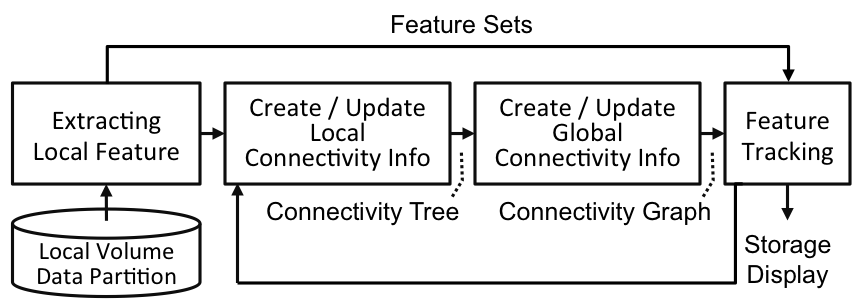
\includegraphics[width=1.0\linewidth]{workflow.png}
\caption{The major steps of our parallel feature extraction and tracking process.}
\label{fig:workflow}
\end{figure}

It is challenging to extract and track features of large time-varying volume data in parallel. First, although a feature can be extracted partially on a processor using the conventional methods, we need to build the connectivity information of the feature across multiple processors. Such information allows us to obtain the global description of a feature from a set of neighboring processors, and enables more advanced operations such as statistical analysis and feature similarity evaluation. Second, such connectivity information can be dynamically changed with features evolving over time. We need to update and maintain the connectivity of features in an efficient fashion to track highly intermittent phenomena.

However, building and maintaining connectivity information of features typically require intensive data exchanges among processors, and thus incurs extra communication cost. To address this issue, we adopt the master-slave paradigm~\cite{Chen03realtime}, but carefully design our parallel feature representation and schedule inter-processor communication to prevent the host from becoming the bottleneck. The local connectivity information is computed and preserved only by the slaves where the correspondent features reside. Hence, there is no global connectivity information maintained at the host. The host only serves as an interface to broadcast the criterion of features to the slaves. In this way, the computation of merging local information is distributed to the slaves. Thus, we can effectively reduce the potential communication bottleneck on the host.

In addition, our approach does not need to set a barrier to wait for all connectivity information to be sent back to the host. Thus, if there exists the features that span over a large number of nodes but are not explored by a user, the potentially long computation time for these features will not block the whole process. This makes it ideal for an interactive system, where users can select the features of interest and instantly receive the visual feedback as the features evolve.

Without loss of generality, for each time step, we partition the volume data into a regular grid of blocks. We then distribute the data blocks among processors, and each processor is assigned with one block.\footnote{Our method can be easily extended to the case that each processor is assigned with multiple data blocks.} In general, a feature can be any interesting object, structure or pattern that is considered relevant for investigation. Here, a feature is defined as the collection of voxels enclosed by a certain iso-surface. Given a sufficiently fine grained partitioning, some features can cross multiple data blocks.

We consider the following two factors in our communication scheme design for better performance and scalability:

\begin{itemize}
	\item $N_{com}$ : The number of communications required to build the connectivity information;
	\item $N_{proc/com}$ : The number of processors involved in each communication.
\end{itemize} 

\subsection{Extracting Partial Local Features}

%------------------------------------------------
\begin{figure}[t]
	\centering
	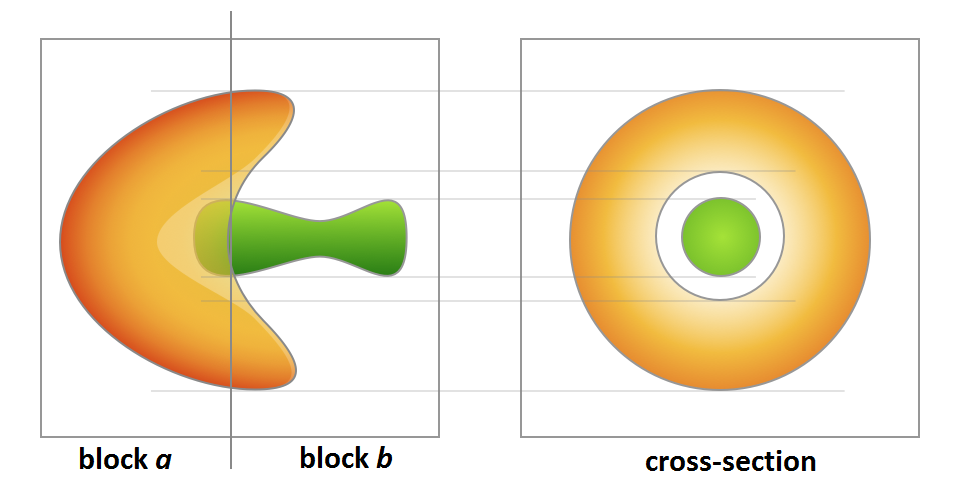
\includegraphics[width=0.9\linewidth]{figure1@2x.png}
	\caption{Two features cross two blocks and share the same centroid on the cross-section.}
	\label{fig:special}
\end{figure}
%------------------------------------------------

Volume features can be extracted using conventional techniques such as region growing, geometry or topology based clustering, or other domain specific algorithms. In this work, we use a standard region-growing algorithm\cite{Lohmann1998} to identify partial features in each data block. This is done by first spreading a set of seeding points inside each data block, and then grow the voxels into a set of separate regions, each regarded as a single feature. As the data is distributed, a feature can cross multiple blocks, and each processor is not aware of the partial features identified on the other processors in this stage. 

\subsection{Matching Partial Local Features}

For the features across multiple blocks, their cross-sections in both sides of the adjacent blocks should match. Therefore, we can connect two partial features by comparing their cross-sections on the corresponding boundary surfaces. That is, two adjacent processors can find the possible matches of the partial features through exchanging and comparing their boundary voxels. Using a ghost area that stores the boundary surface belonging to a neighbor may help to achieve voxel-wise matching for the partial features. However, maintaining such ghost areas requires frequent inter-process communication and is considerably expensive for interactive applications. 

To reduce communication cost and accelerate comparison, we use a simplified method to detect matches. We first represent the cross-section on a boundary surface as:

\begin{itemize}
	\item $P_{centroid}$: The geometric centroid of the cross-section of the feature;
	\item $P_{min}$ and $P_{max}$: The minimal and maximal coordinates of the cross-section area.
\end{itemize}

%------------------------------------------------
\begin{algorithm}[t]
\caption{Match of two partial features $f$ and $f^{'}$}
	\begin{algorithmic}
		\IF{$abs(P_{centroid} - P_{centroid}^{'}) \leq 1$ 
		\textbf{and} $abs(P_{min} - P_{min}^{'}) \leq 1$ 
		\textbf{and} $abs(P_{max} - P_{max}^{'}) \leq 1$}
			\STATE return $f$ \textbf{matches} $f^{'}$
		\ENDIF
	\end{algorithmic}
\label{alg:match}
\end{algorithm}
%------------------------------------------------

For two partial features, we then compare their geometric centroids. If the difference is larger than 1-voxel offset, we consider that they belong to different features. However, only considering geometric centroids is not sufficient to match two features. In some special cases, two different features can have the same geometric centroid on the boundary surface, as shown in Figure~\ref{fig:special}. Therefore, we also need to consider the min-max coordinates of the cross-section areas to detect bipartite matching of partial features, as shown in Algorithm~\ref{alg:match}. In this way, we only need to exchange 3 coordinate values, which, in most cases, are sufficient to detect feature connection across a boundary in practice.

\subsection{Creating Local Connectivity Tree}

Based on our method to match the partial local features, we can abstract the local connectivity information using a tree structure. As shown in Figure~\ref{fig:match}. each data block has six direct neighbors (the outermost blocks have less), each with a shared boundary surface. The connectivity tree is constructed by taking the block as root and its six adjacent blocks as its first level child nodes. A leaf is appended to a first level node if and only if a local feature touches the corresponding boundary surface. Note that a feature can touch multiple boundary surfaces and thus be attached to multiple first level nodes.

Each voxel in the local data block has a unique global index, and thus each leaf can be encoded using 3 integers (global index for $P_{centroid}$, $P_{min}$ and $P_{max}$). We use $P_{centroid}$ as the feature index, and sort the sibling leaves according to the indexes in ascending order. In addition, the root and the first level child nodes can be encoded with the indexes of corresponding data blocks, which are irrelevant to the number of features-on-boundary (henceforth referred as $N_{fb}$). Therefore, the overall spatial complexity of a local connectivity tree for each data block is $\theta(3*N_{fb})$, which is typically negligible compared with the volume size. 

%------------------------------------------------
\begin{figure}[t]
	\centering
	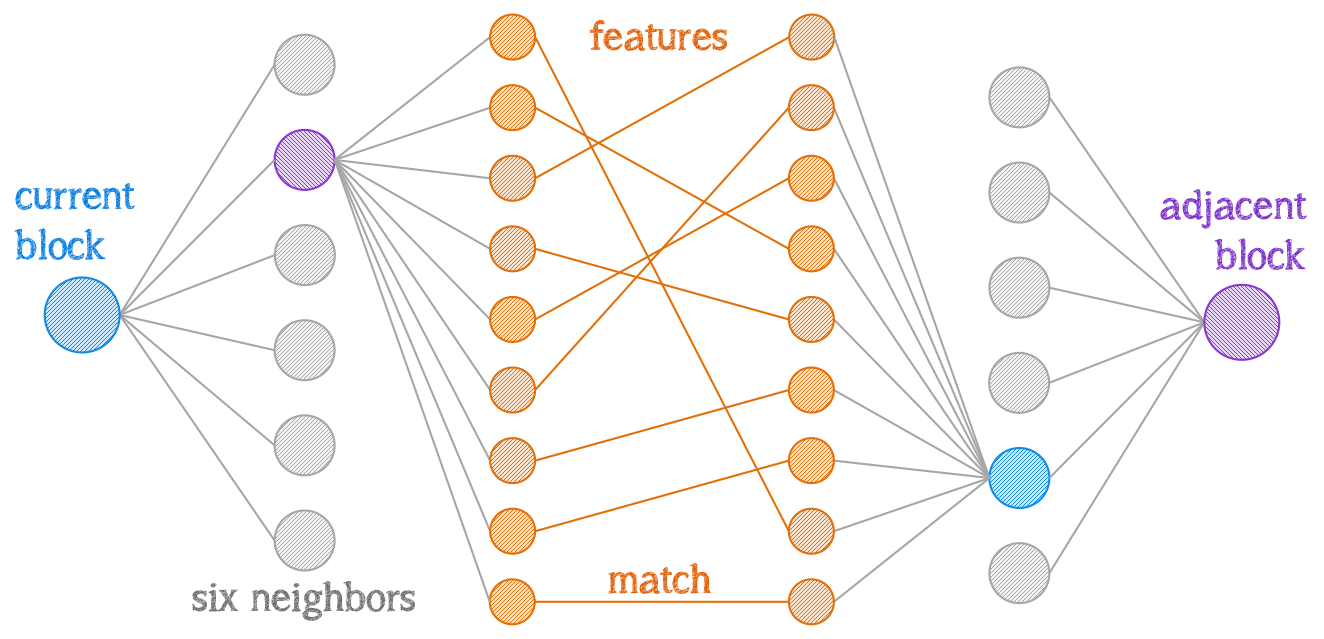
\includegraphics[width=1\linewidth]{match.png}
	\caption{Top: Two blocks with four features across the blocks. Bottom: The tree structure used for maintaining local connectivity information, where the root node is encoded with the block index, its child nodes are encoded with the indexes of its neighboring blocks, and the leaves of each first level child node represent the local partial features. The leaves should match the ones residing on the corespondent neighboring block, which are indicated by the dashed lines.}
	\label{fig:match}
\end{figure}
%------------------------------------------------

From the perspective of temporal complexity, the creation of a local connectivity tree does not introduce an extra computational cost as it can be done along with the region growing process. The values of $P_{centroid}$, $P_{min}$ and $P_{max}$ are updated only if a feature reaches the boundary surface.

\subsection{Creating Global Connectivity Information}

After a local connectivity tree is created within each data block, their leaves need to be exchanged and merged to obtain the overall description of a partitioned feature. The exchanging and merging process is decisive in that its effectiveness largely affects the overall performance and scalability of the feature tracking algorithm as a whole.

\subsubsection{Representation of Connectivity Information}

Based on the tree structure of the local connectivity information, the global connectivity information can be described as a graph that connects the local connectivity trees, as shown in Figure~\ref{fig:match}. To facilitate data exchanges among processors, we adopt the linear representation techniques~\cite{AMET1990} and represent the global connectivity information into a feature table. Each feature has a global unique ID. The table is indexed by the feature IDs, and each entry lists the processors that contains the corresponding partial local features. Given this simple representation, once a user selects a feature, each related processor can query the table to identify the other processors that need to be communicated to collectively operate on the selected feature.

\subsubsection{The Centralized Approach}

One possible solution to build the global feature table is to directly use the master-slave paradigm. When the feature extraction process is done, all local connectivity trees are gathered to the host processor. Then the host starts to merge the leaves from each connectivity tree and matches the partial features to build the global feature table.

The merit of this centralized approach lies in that it requires inter-processor communication only once; that is, $N_{com} = 1$ for each processor. Moreover, the global feature table can be preserved in the host that it can directly respond to feature queries without collecting information from the slaves again. However, this approach has an obvious drawback. Since all local connectivity trees are sent to the host, the number of processors involved in each communication is $N_{proc/com} = N_p$, and there exists potential contention, both in communication and computation, on the host.

\subsubsection{The Decentralized Approach}
\label{sec:decentralized}

A better solution is to decentralize the gathering and merging process from using a single host processor to exploiting all available processors. After the feature extraction process is done and so does the creation of local connectivity tree, an \emph{all-gather} process starts to exchange all local connectivity trees among processors. Each processor first collects a full copy of all local trees and merges the leaves to obtain the global feature table. However, this approach does not actually resolve the contention problem since every processor acts like the host and it still needs to gather and merge all local trees. 

%------------------------------------------------
\begin{figure}[t]
	\centering
	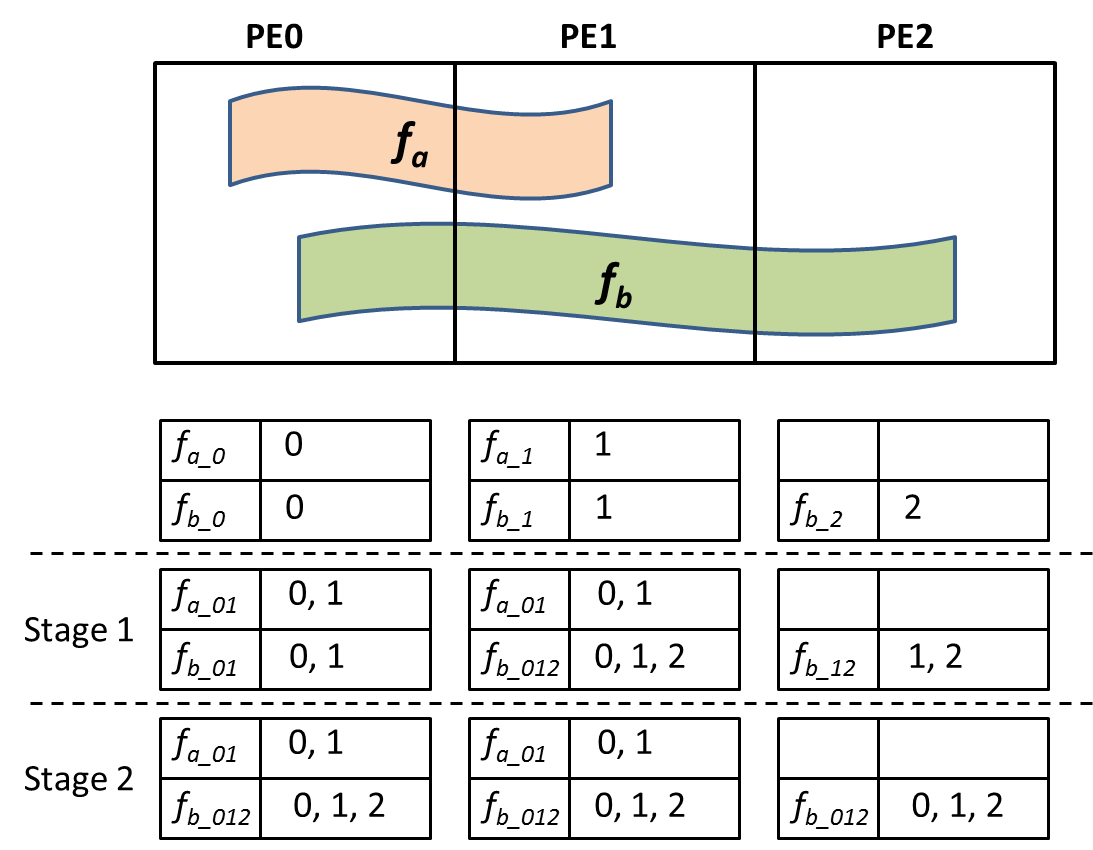
\includegraphics[width=0.9\linewidth]{global_feature_table.png}
	\caption{Construction of partial global feature table with three processors and two features. There are two communication stages. At each stage, each processor only communicates with its immediate neighbors. Each entry of the table is indexed by the feature IDs and lists the processors that contain the corresponding feature.}
	\label{fig:global_table}
\end{figure}
%------------------------------------------------

We observe that, for a real-world data set, it is rarely the case that all features are spanning over every data block. In addition, it is unnecessary for each processor to construct a global feature table to contain all features. Each processor only needs to construct a partial table that records the other processors sharing the same set of features. Thus, it is possible for a processor to communicate with a small set of processors to construct the needed portion of the table. However, on the other hand, we also observe that each processor has no information of the partial features identified on the other processors. Thus, initially, a processor is not aware of other processors with which can be directly communicated to gather the partial features. 

Based on these observations, we design an iterative approach that uses a multi-stage communication scheme. During each stage, each processor only communicates with its immediate neighbors to exchange and propagate the feature connectivity information. This could be considered as a higher level of region growing process that starts from one seeding block and grows to adjacent blocks by exchanging and merging connectivity information in a breadth-first fashion, until all cross-boundary features are connected. 

Figure~\ref{fig:global_table} gives an example of the procedure to construct a partial global feature table with three processors and two features.\footnote{For simplicity, we use an example of 1D partitioning. However, the procedure can be easily extended to 3D cases.} We can see that the feature $f_a$ is identified by the processors PE0 and PE1, and the feature $f_b$ is identified by PE0, PE1 and PE2. Initially, each processor constructs a partial global feature table initialized with only the local features with their local IDs, such as $f_{a\_0}$, $f_{b\_2}$, and so on. In the first stage, PE0 exchanges the local connectivity tree with PE1, and PE1 exchanges the tree with PE2. After exchanging trees, each processor independently matches the partial features, and updates the corresponding feature IDs and entries in its table. For example, the ID of $f_a$ has been changed to $f_{a\_01}$ on both PE0 and PE1, and the entry contains the same processor list. However, for $f_b$, as the information has not been propagated between PE0 and PE2, its ID is different on the three processors. In the second stage, each processor still only communicates with its immediate neighbors, and the information of $f_b$ has been propagated to PE0 and PE2 through PE1. Thus, for $f_b$ ID and its processor list are all the same on the three processors. After an extra communication, each processor detects there is no further information sent from its neighbors, and thus the construction of the partial global feature table is completed.

After constructing its partial global connectivity table, for any selected features, each processor can easily find other corresponding processors. For example, in Figure~\ref{fig:global_table}, if $f_a$ is selected, PE0 and PE1 can mutually find that each other belongs to the same communicator, while PE2 is excluded.

The reason we choose the six-direct-neighbor paradigm is because it can minimize the communication cost. It takes a maximum of ${3n-1}$ times communications, where $n$ denotes the maximum processor number among the axes. This corresponds to the maximum communications needed for propagating the information of a feature that covers the whole domain, although this case is nearly impossible in practice. The temporal complexity for garnering all necessary leaves is hence as low as ${O(\sqrt[3]{N_{proc}})}$. And the number of processors involved in each communication is a constant of a maximum of six, i.e., $N_{proc/com} \leq 6$.

Another optional paradigm is to let each processor communicate with its 26 neighbors, including the adjacent diagonal blocks. Communication with the adjacent diagonal block takes as much as half the time for any block to reach its furthest diagonal. However, $N_{proc/com}$  is also increased to 26. For data sets where features only span over a small number of blocks, the 6-direct-neighbor paradigm outweighs the 26-neighbors paradigm in communication complexity.

\subsection{Updating Global Connectivity Information}

%------------------------------------------------
\begin{figure}[t]
	\centering
	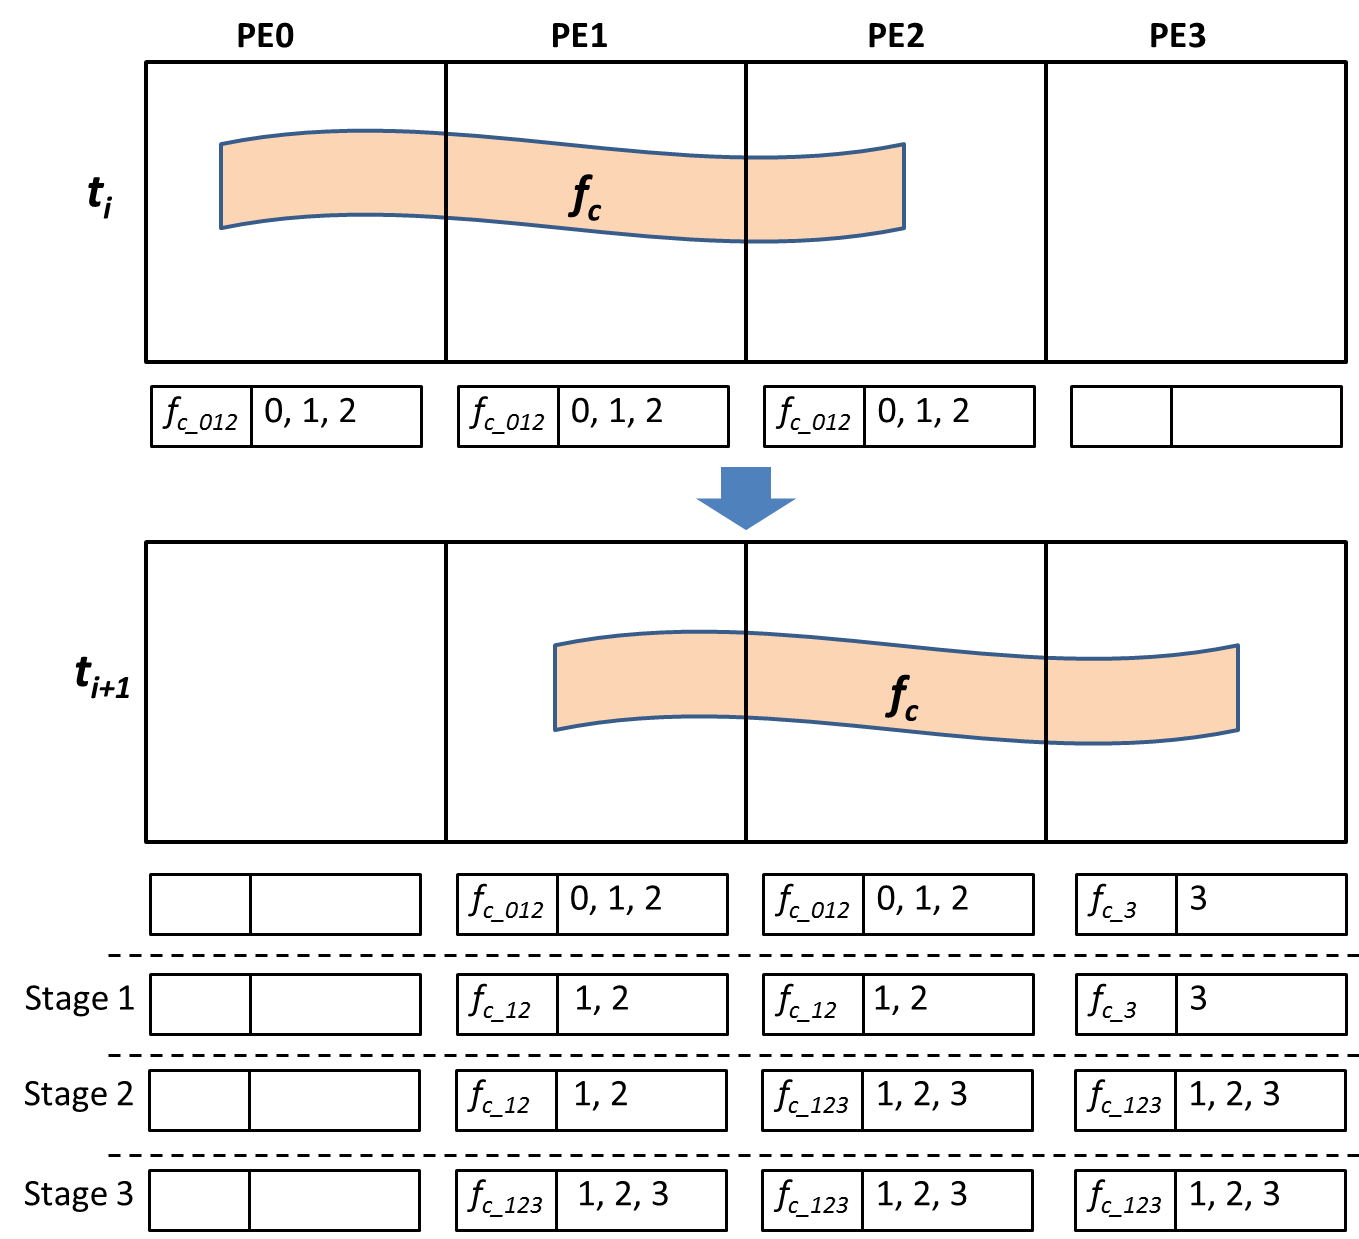
\includegraphics[width=1\linewidth]{global_grow_feature_table.png}
	\caption{Update of partial global feature table with four processors and one feature. Feature $f_c$ is extracted and adjusted in Stage 0 followed by three communication stages to record the possible shrinking and expanding of the feature. }
	\label{fig:hybrid}
\end{figure}
%------------------------------------------------

To track features, we can construct the global connectivity table for each time step. However, if the time interval is sufficiently small for generating the data, volumetric features may drift but should not change drastically in neither size, shape, nor location. We assume that the changes of each feature are within the range of one block. Based on this assumption, we can optimize feature tracking by incrementally updating the global connectivity information over time.

As depicted in Figure~\ref{fig:hybrid}, each processor constructs a partial global feature table at time step $t_i$. Meanwhile, we maintain a communicator, $\textbf{C}$, which contains the corresponding processors for each feature. For example, feature $f_c$ spans over PE0, PE1, and PE2. These three processors have the same table entry with respect to $f_c$. The table of PE3 is empty at $t_i$. PE0, PE1 and PE2 belong to the same communicator $\textbf{C}$.

For the next time steps, $t_{i+1}$, each processor continues to predict and correct boundaries as to extract partial local features. For the existing features, their IDs are retained in the partial global feature table. For the new features, their IDs are added into the table. And the IDs are erased from the table if the corresponding features drift away from that block. As shown in Figure~\ref{fig:hybrid}, $f_c$ leaves PE0 and enters PE3. In this case, the table of PE0 becomes empty, and the table of PE3 adds a new entry. At this time point, the feature ID on PE3 is not the same as the others, as the feature has not been matched yet. In addition, PE0, PE1 and PE2 still belong to $\textbf{C}$. 

Then we start to update the connectivity information. In the first stage, PE0, PE1, and PE2 perform an \emph{all-gather} operation within their communicator $\textbf{C}$ to update the connectivity. PE0 is then removed from the corresponding entry on PE1 and PE2, and also removed from $\textbf{C}$. In the second stage, each processor exchanges the local connectivity information with the immediate neighbors as the decentralized approach in Section~\ref{sec:decentralized}. The information of $f_c$ is propagated between PE2 and PE3. In the third stage, all the processors in the communicator $\textbf{C}$ perform an \emph{all-gather} operation again to update the connectivity. The information of $f_c$ is propagated to the rest of processors $\textbf{C}$, and then PE1, PE2, and PE3 have the same table at $t_{i+1}$. Given the unified information, we can then update the communicator $\textbf{C}$ by including PE3 with respect to $f_c$. 

This update procedure can be easily extended to the circumstances with more processors and features. We note that the cost of collective communication is marginal within a communicator of limited size. By leveraging this nice property, for each feature, we only need at most three stages to update the connectivity information, independent of the length of the feature.
%------------------------------------------------------------------------------

%------------------------------------------------------------------------------
%-------------------------------------------------------------------------
\begin{figure}[t]
% 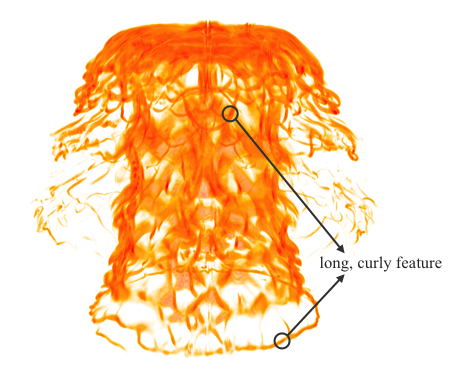
\includegraphics[width=0.49\linewidth]{combustion_labeled.png}
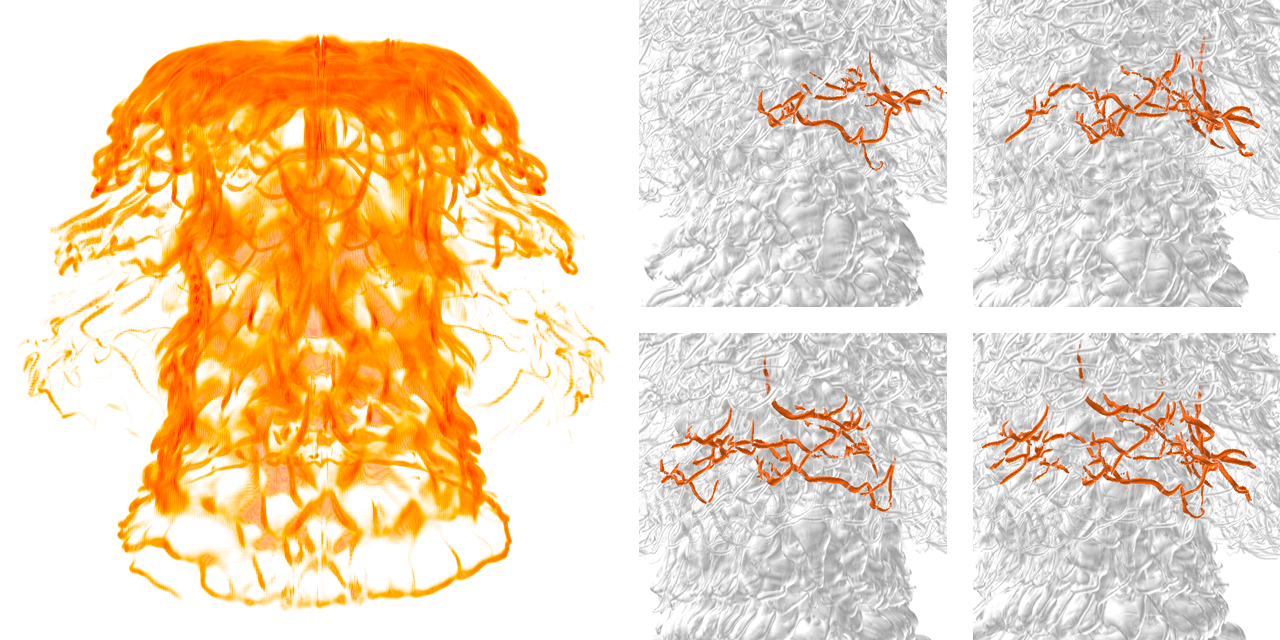
\includegraphics[width=1.0\linewidth]{combustion_ft.png}
% 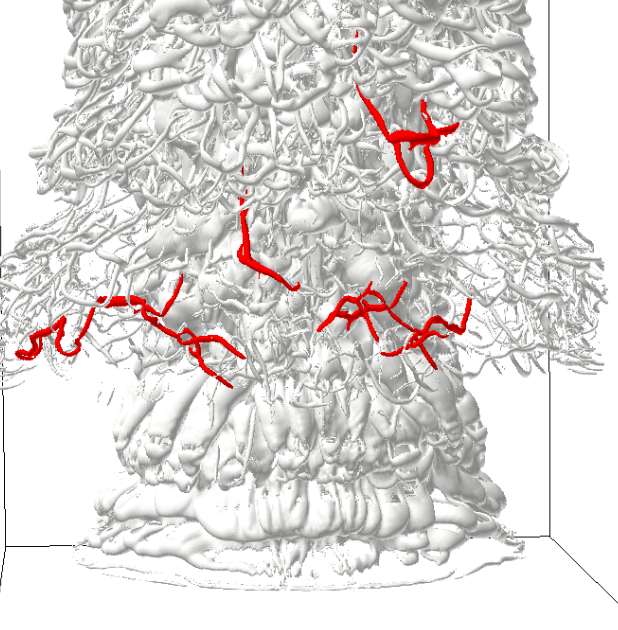
\includegraphics[width=0.49\linewidth]{combustion_feature.png}
\caption{Left: The volume rendering of a single time step of the combustion data set; Right: Selected features of interest extracted tracked overtime.}
\label{fig:combustion-labeled}
\end{figure}

\begin{figure}[t]
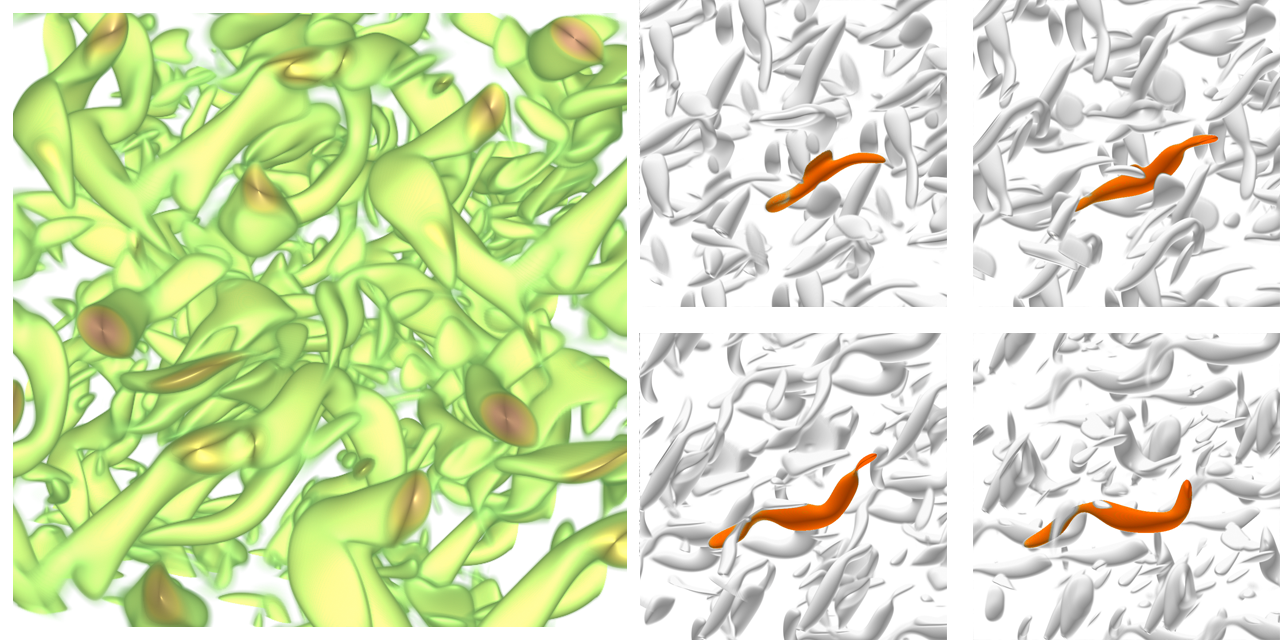
\includegraphics[width=1.0\linewidth]{vorts_ft.png}
% 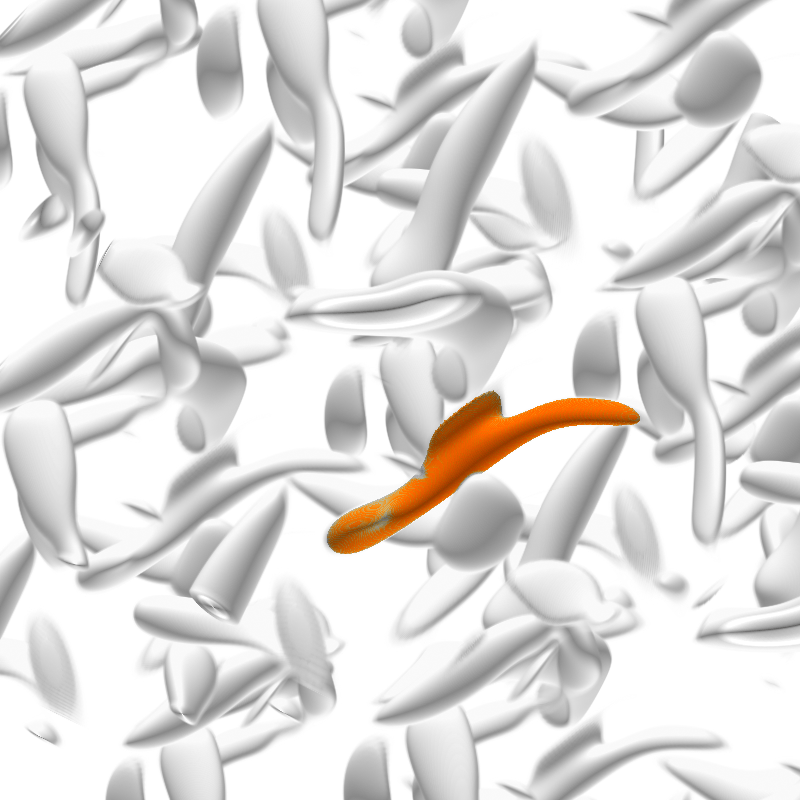
\includegraphics[width=0.24\linewidth]{vorts1.png}
% 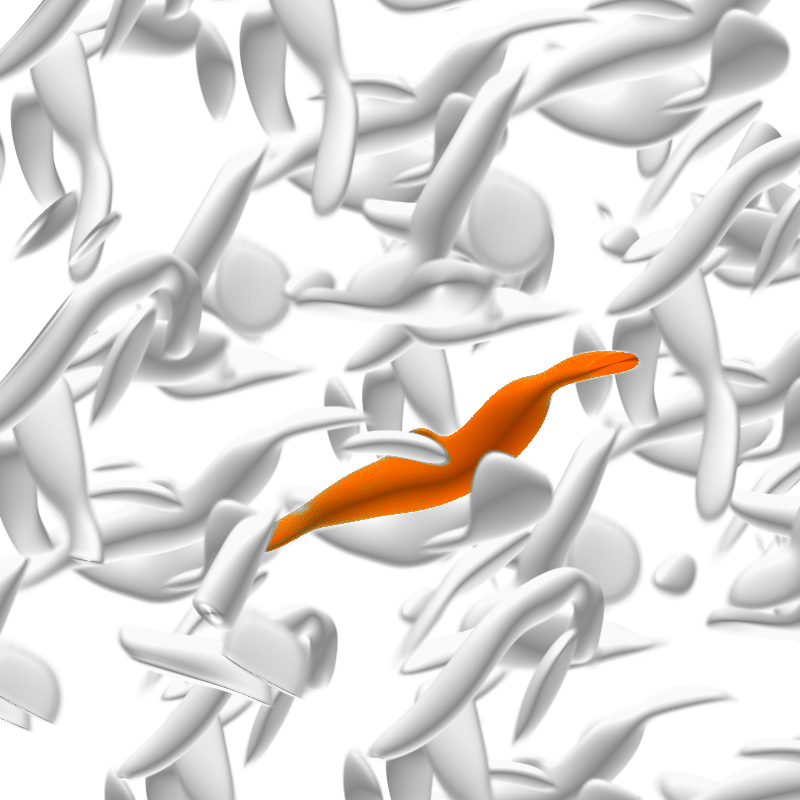
\includegraphics[width=0.24\linewidth]{vorts3.png}
% 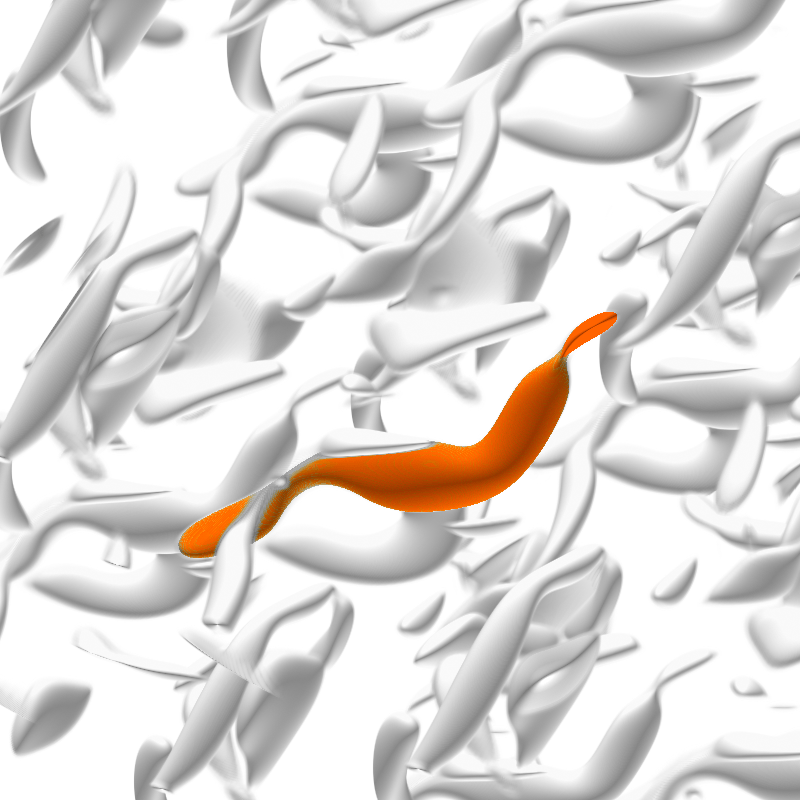
\includegraphics[width=0.24\linewidth]{vorts5.png}
% 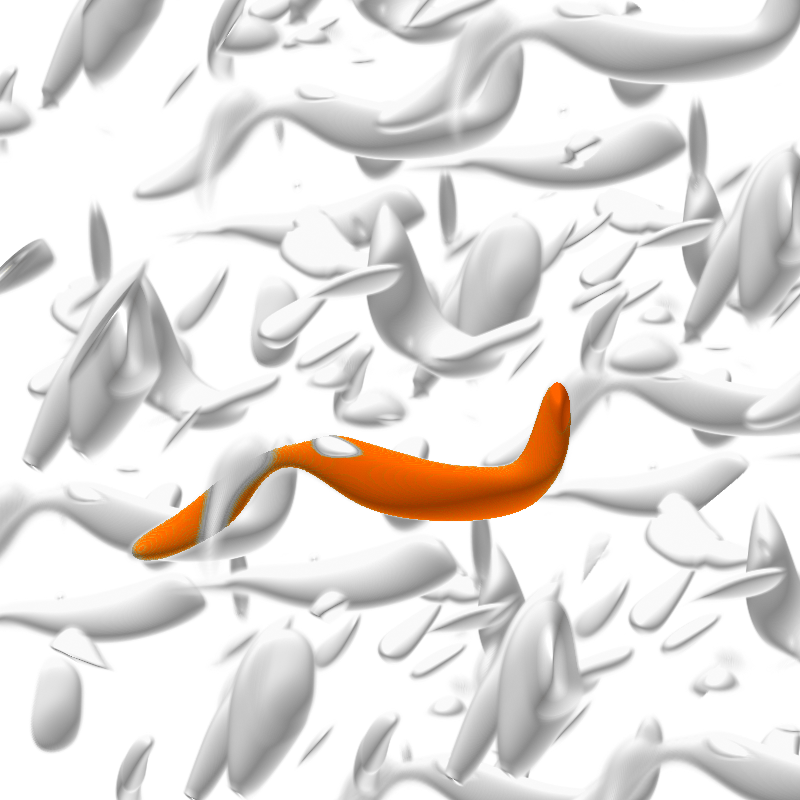
\includegraphics[width=0.24\linewidth]{vorts7.png}
\caption{Left: The volume rendering of a single time step of the vortex data set; Right: Selected features of interest extracted tracked overtime.}
\label{fig:vorts-tracking-result}
\end{figure}
%-------------------------------------------------------------------------

\section{Results}

We test our feature extraction and tracking algorithm on two datasets. A 400 time steps $256\times256\times256$ vortex data set obtained from a combustion solver that can simulate turbulent flames, and a 100 time steps $1024\times1024\times1024$ vortex data set synthesized from the $128\times128\times128$ volume data set used in the other works~\cite{Silver:1997:TVT:614266.614369, Ji2003, Ji2006}. In the combustion data set, each voxel contains the magnitude value of vorticity derived from velocity using a curl operator. As time evolves, vortical features may vary from small amassed blob features to long curly features that span over large portion of the volume. Figures~\ref{fig:combustion-labeled} and \ref{fig:vorts-tracking-result} show the examples of identified and tracked features in these two data sets.

Since our design is to target an in situ setting, we ignore the I/O cost and only focus on the computation time in our study.

%\subsection{Performance Result}

% The volume data can be generated either in advance or on the fly, and thus we ignore the I/O cost and only focus on the computation time for the following three portions.


\textbf{Time for extracting features ($T_{extract}$).}
%
Since we use the region-growing based algorithm to extract features, given a fix specification of features, the computation time is mainly determined by the size of the volume as well as the number of processors being used. Once the raw volume data and its partitioning, a.k.a. the size of each data block is determined, the computation time for extracting residing features remains approximately the same. In post-processing, the size of each data block decreases with the increasing number, and hence so does the time spent on extracting features. As depicted in Figure~\ref{fig:feature-extraction}, $T_{extract}$ is approximately log-linear decreased as the number of processors increases.

\begin{figure}[t]
\centering
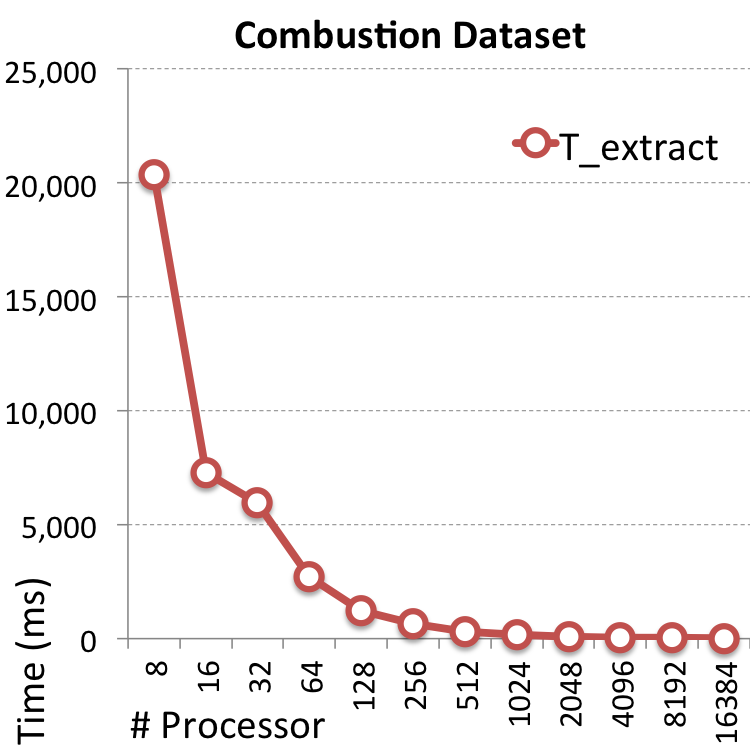
\includegraphics[width=0.49\linewidth]{combustion_t_extract.png}
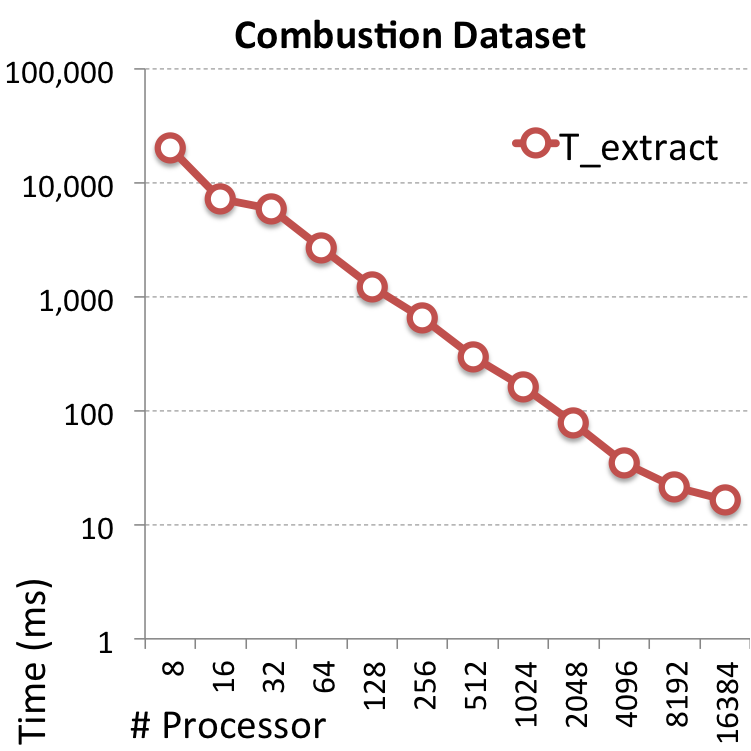
\includegraphics[width=0.49\linewidth]{combustion_t_extract_log.png}
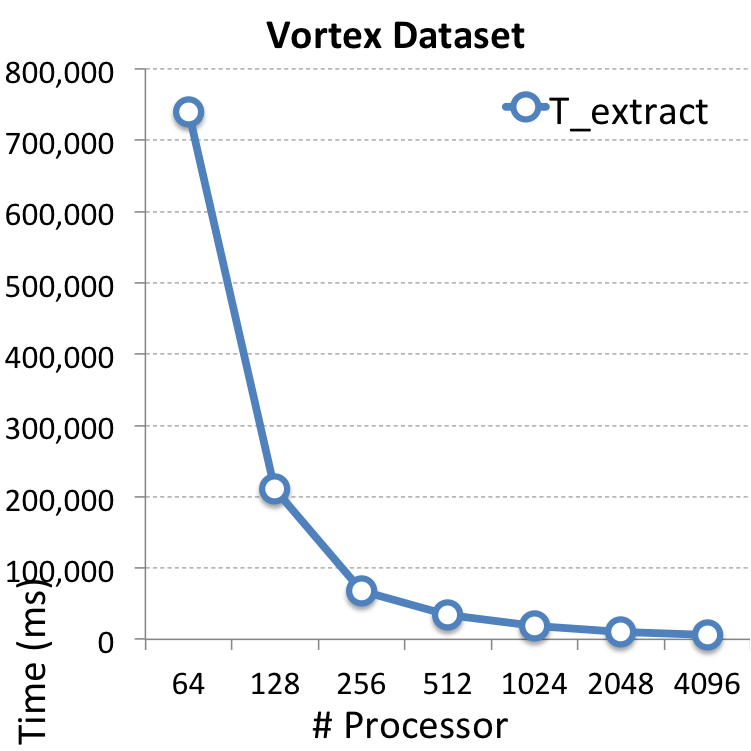
\includegraphics[width=0.49\linewidth]{vorts_t_extract.png}
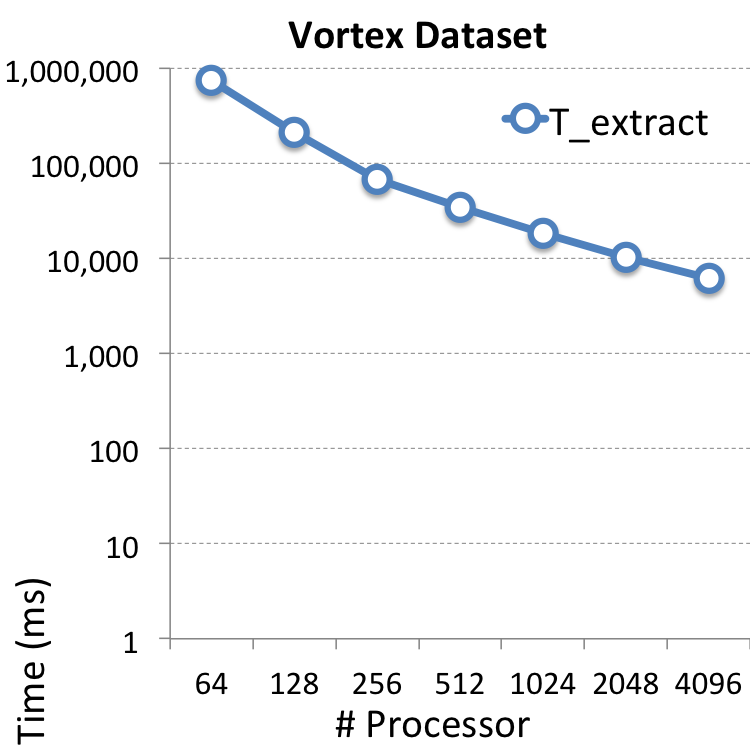
\includegraphics[width=0.49\linewidth]{vorts_t_extract_log.png}
\caption{Computation time for feature extraction. The left two plots are shown in linear scale, and the right plots are shown in logarithmic scale. The speedup is linear with the number of processors.}
\label{fig:feature-extraction}
\end{figure}

\textbf{Create Local Connectivity Tree ($T_{create}$).}
%
Despite the size of each data block, the computation cost for creating and updating local connectivity tree is dependent on the number of the features extracted within the original volume, or more precisely, the number of features that touches the boundary surface of their residing data block. As shown in Figure~\ref{fig:create-local-graph}, similar to $T_{extract}$, $T_{create}$ decreases as the number of processors increases in post-processing, as the the number of feature-on-boundary decreases accordingly. For both the combustion and vorticity data set, it takes an average of 0.1 seconds to create the local connectivity tree, approximately 0.5\% the time of $T_{extract}$ using the same amount of processors. This portion increases but does not succeed 1\% in out test, hence $T_{create}$ is not considered as a bottleneck. %\textcolor{red}{for in-situ visualization however... }

\begin{figure}[t]
\centering
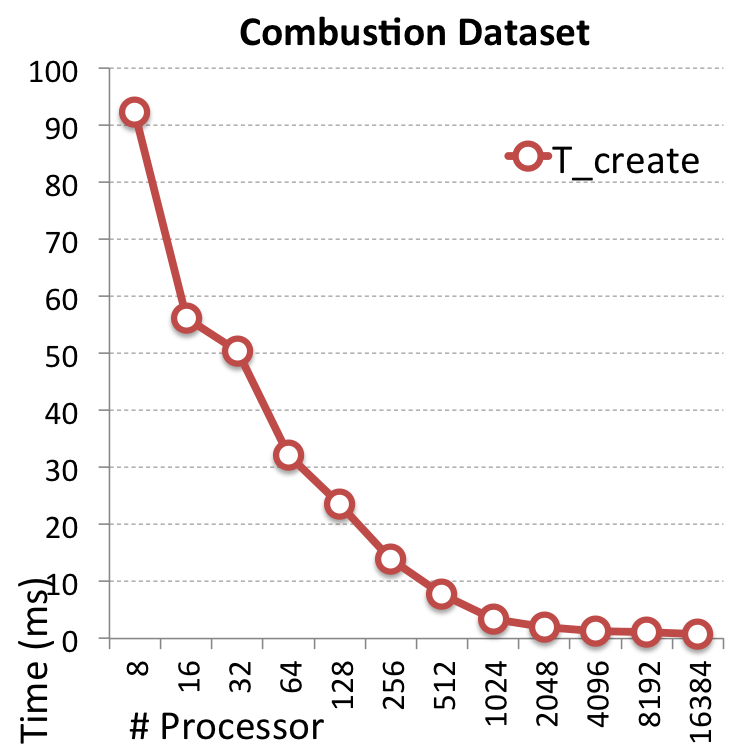
\includegraphics[width=0.49\linewidth]{combustion_t_create.png}
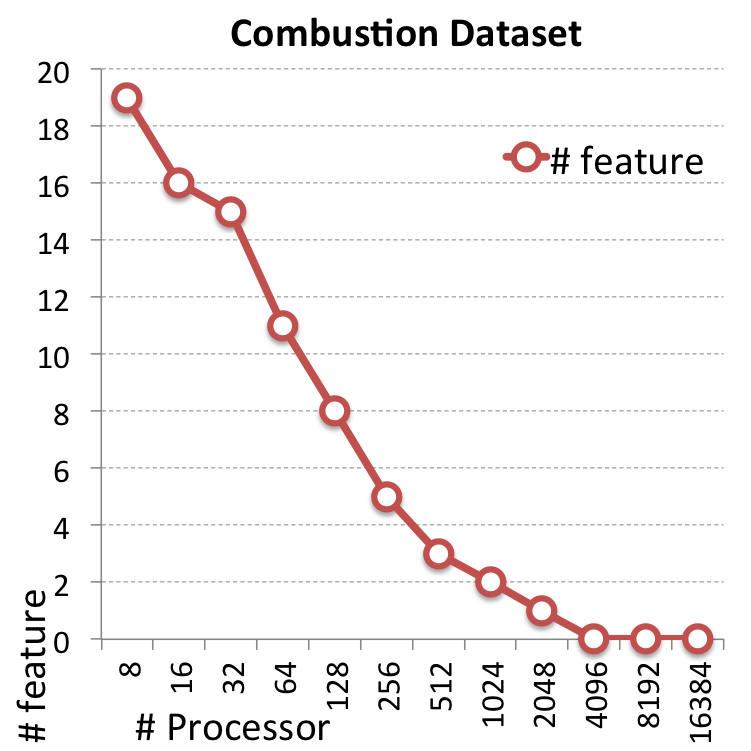
\includegraphics[width=0.49\linewidth]{combustion_num_feature.png}
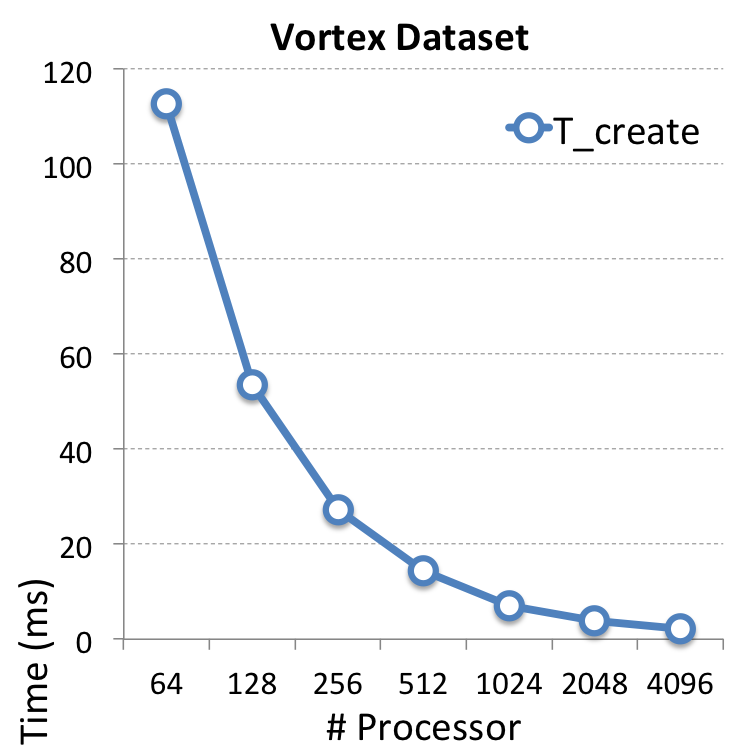
\includegraphics[width=0.49\linewidth]{vorts_t_create.png}
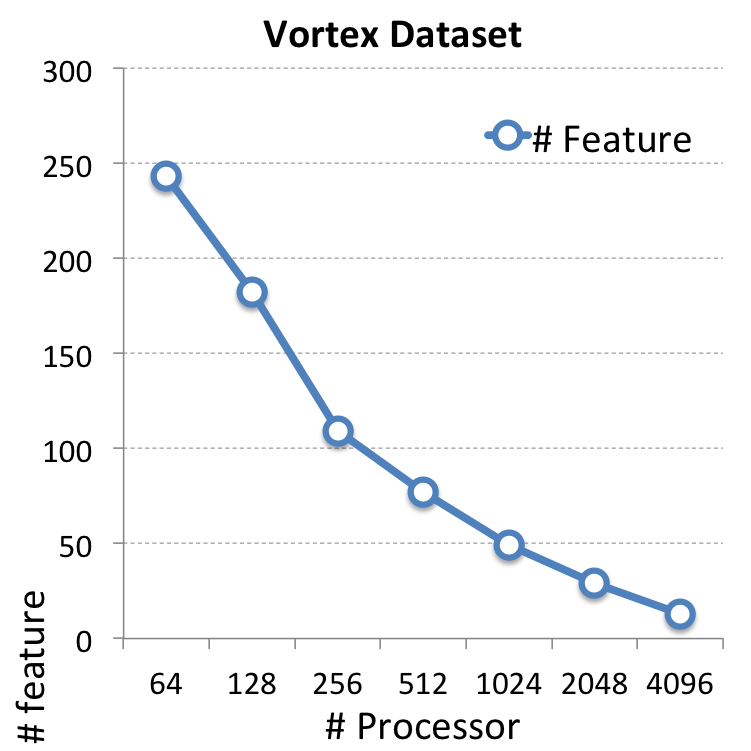
\includegraphics[width=0.49\linewidth]{vorts_num_feature.png}
%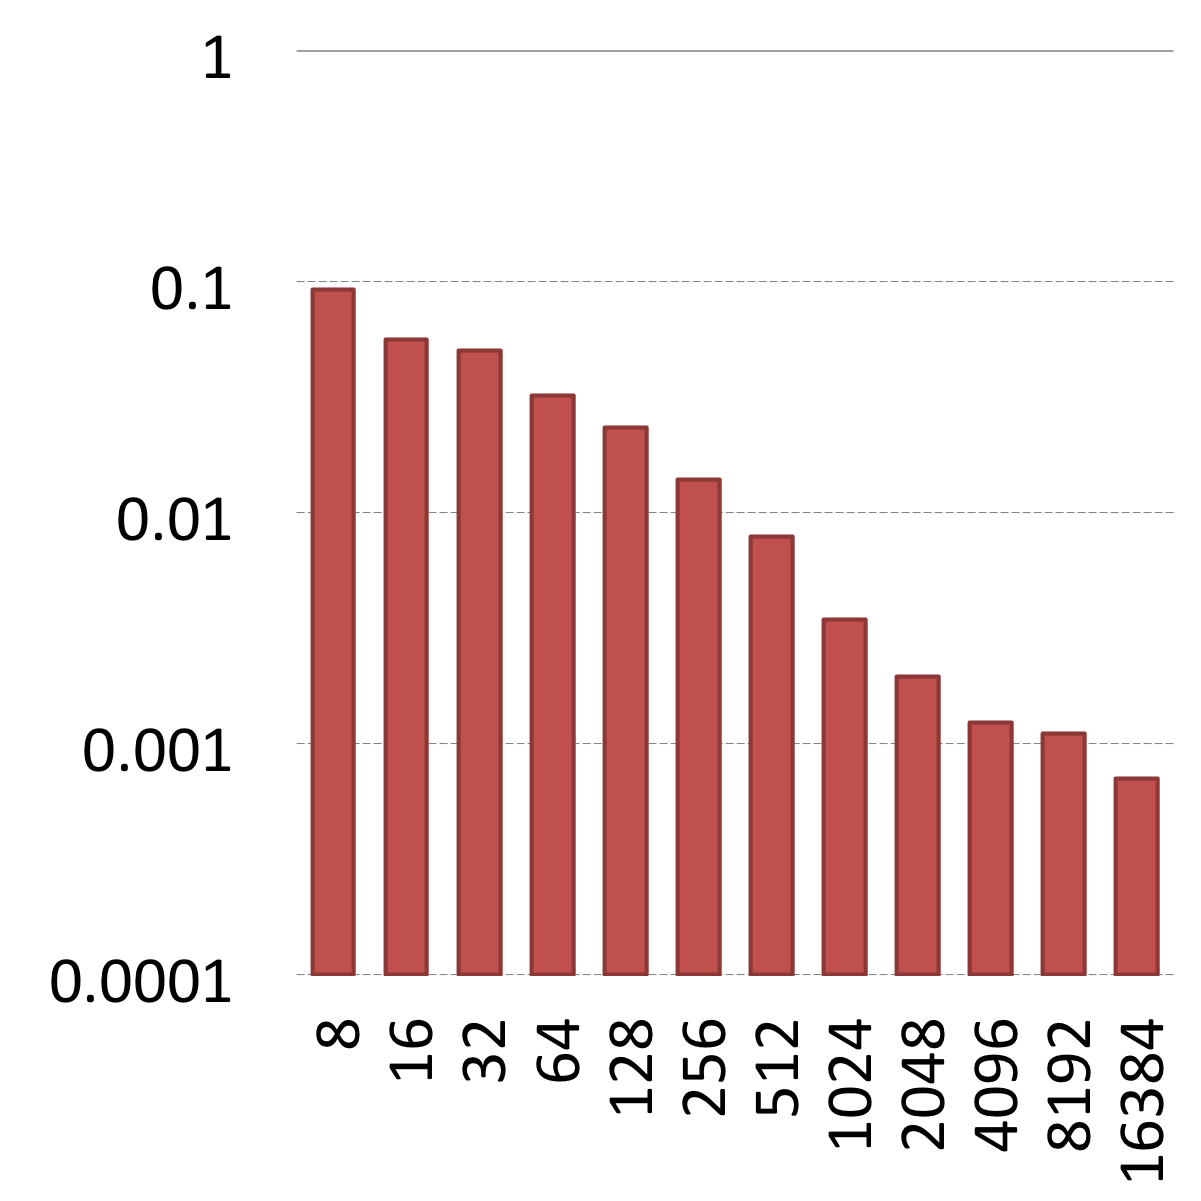
\includegraphics[width=0.6\linewidth]{create_local_graph_log.png}
\caption{Computation time for creating local connectivity tree. The speedup is linear with the number of processors. And the time cost is approximately proportional to the number of features-on-boundary. Note that, for the processor number greater than 4096 for the combustion data set and 512 for the vorticity data set, the average feature number is between 0 and 0.5 and is rounded to 0.}
\label{fig:create-local-graph}
\end{figure}

\begin{figure}[ht]
\centering
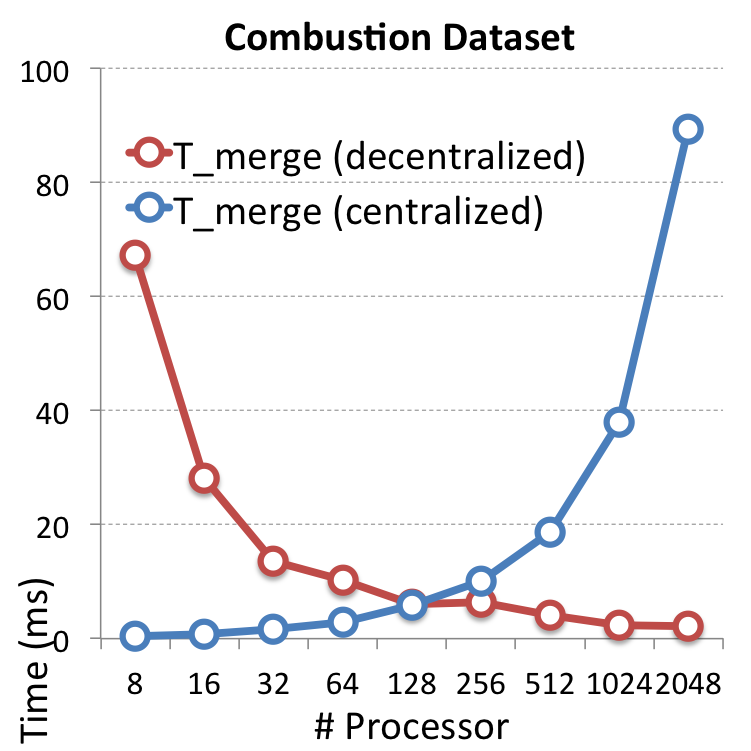
\includegraphics[width=0.45\linewidth]{combustion_local_vs_global.png}
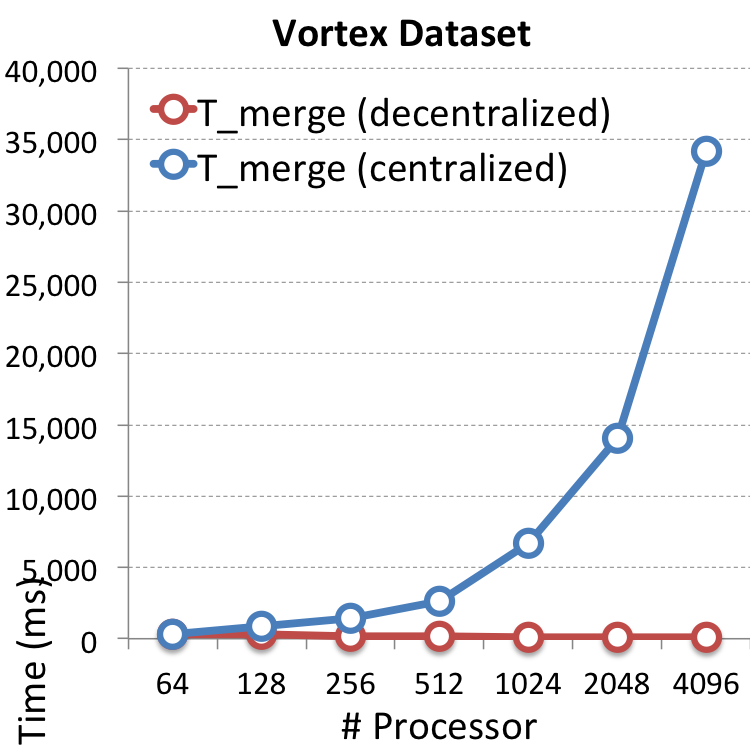
\includegraphics[width=0.45\linewidth]{vorts_local_vs_global.png}
\caption{The comparison between the computation time for the centralized approach and the decentralized approach. The centralized approach works well for a small number of processors while the decentralized approach exceeds after a certain number, e.g. 128 processors for the combustion data set, is used.}
\label{fig:local-vs-global}
\end{figure}

% Total computation time comparison for different approaches to
% global connectivity information generation. The centralized approach
% scales up to 2048 processors but the merging time outweighs
% the extraction time when using more processors;
% The decentralized approach scales linearly
% up 16384 processors for the combustion data set.

\begin{figure}[t]
\centering
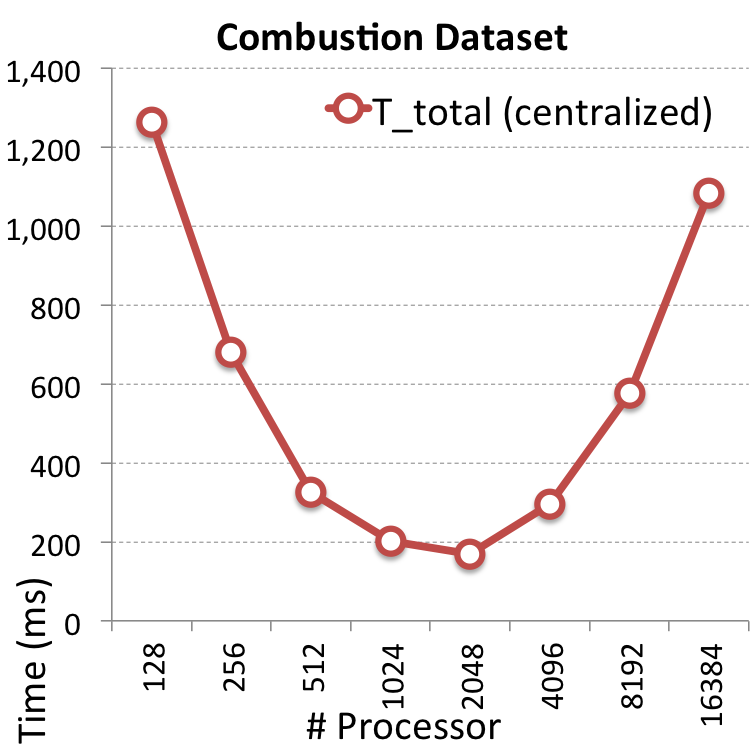
\includegraphics[width=0.49\linewidth]{combustion_t_total_centralized.png}
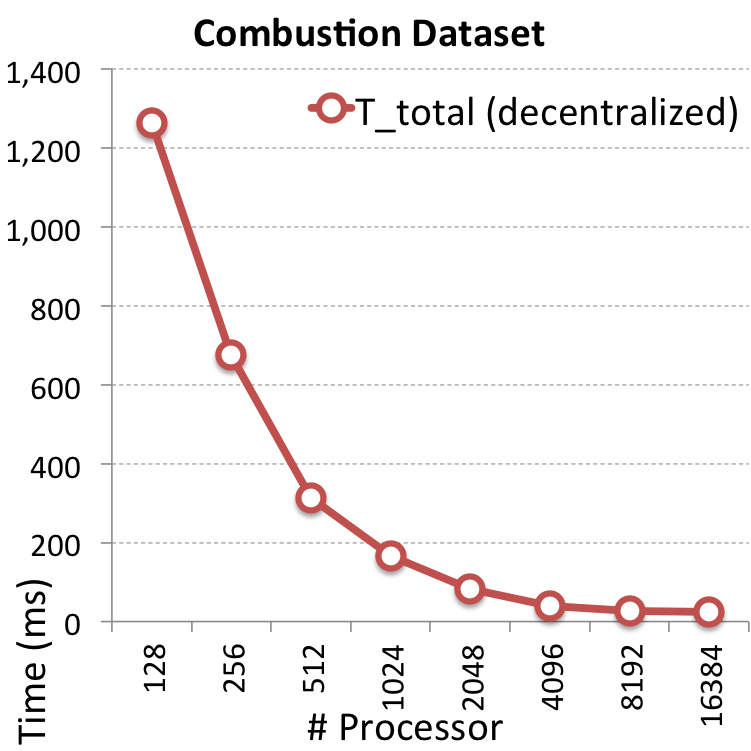
\includegraphics[width=0.49\linewidth]{combustion_t_total_decentralized.png}
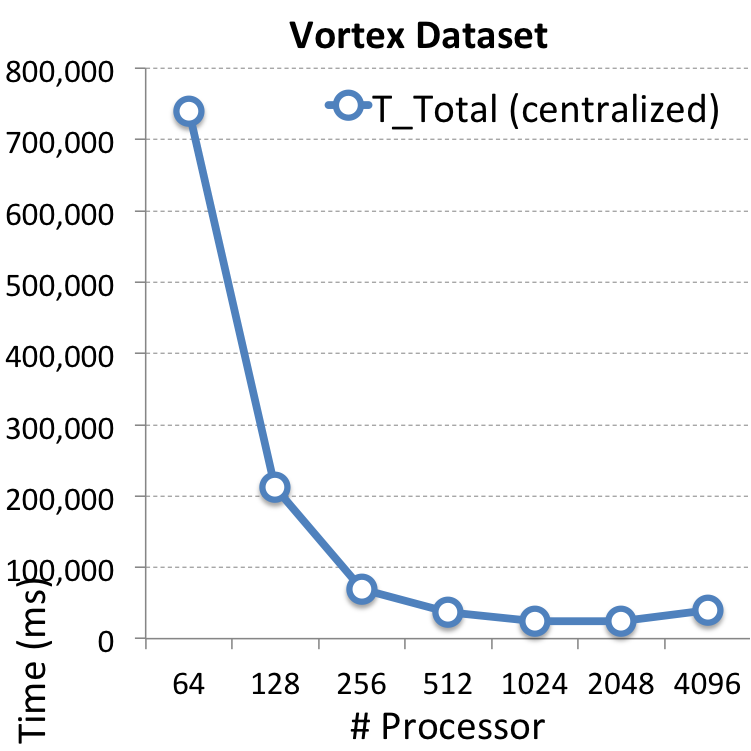
\includegraphics[width=0.49\linewidth]{vorts_t_total_centralized.png}
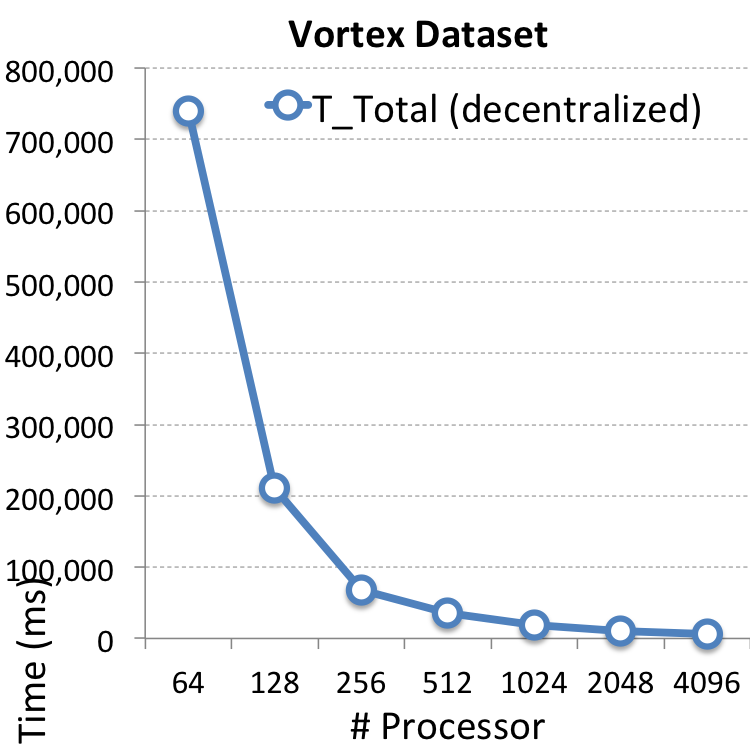
\includegraphics[width=0.49\linewidth]{vorts_t_total_decentralized.png}
% 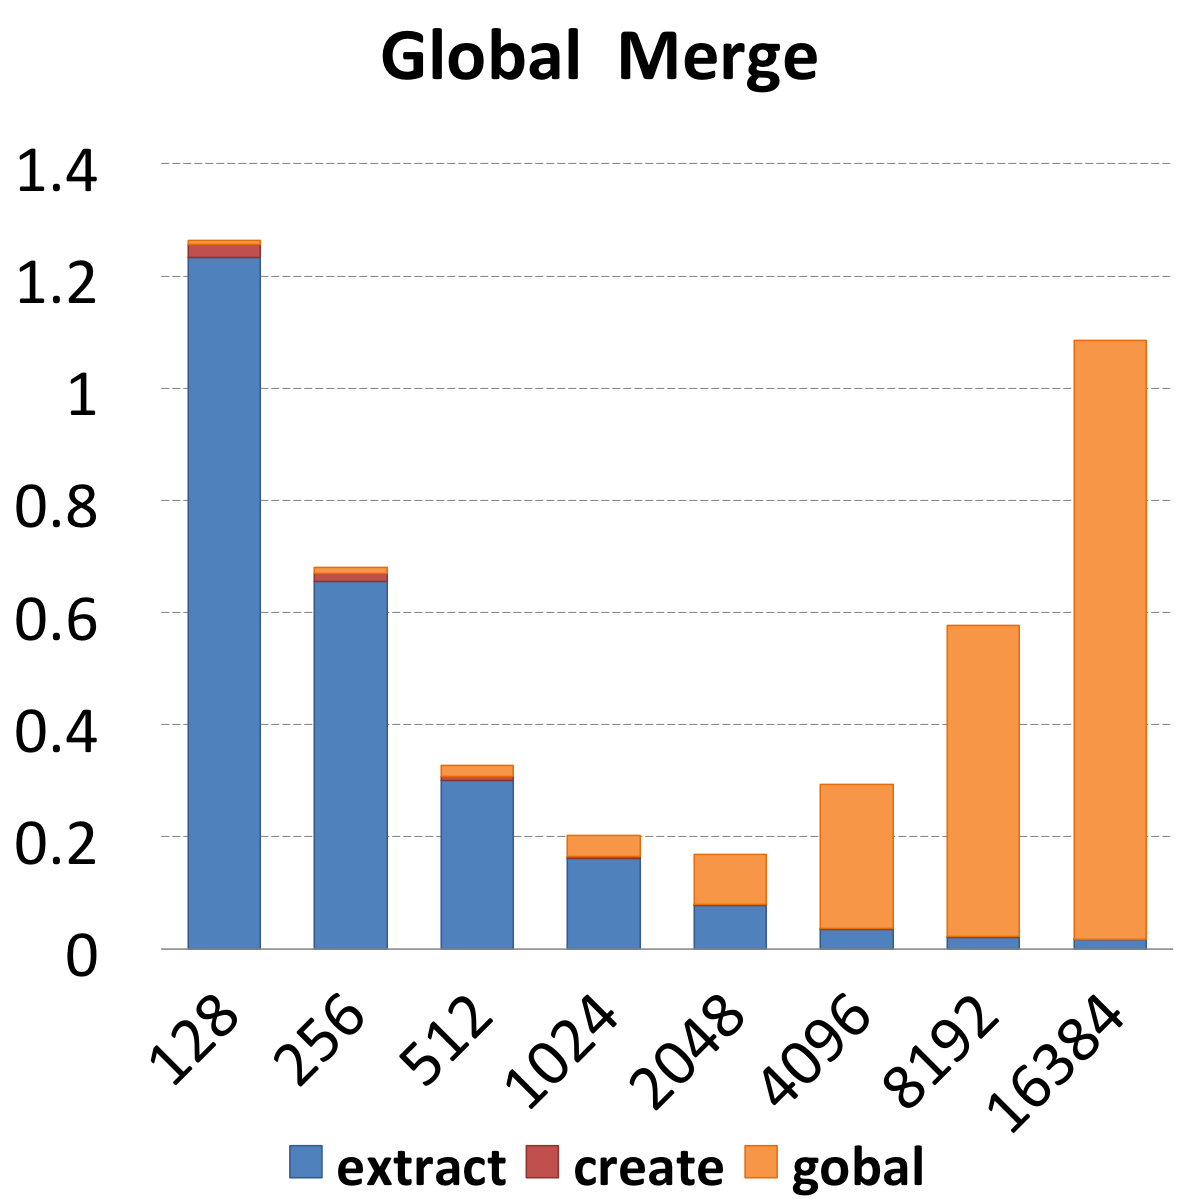
\includegraphics[width=1.0\linewidth]{global_merge.png}\\
% 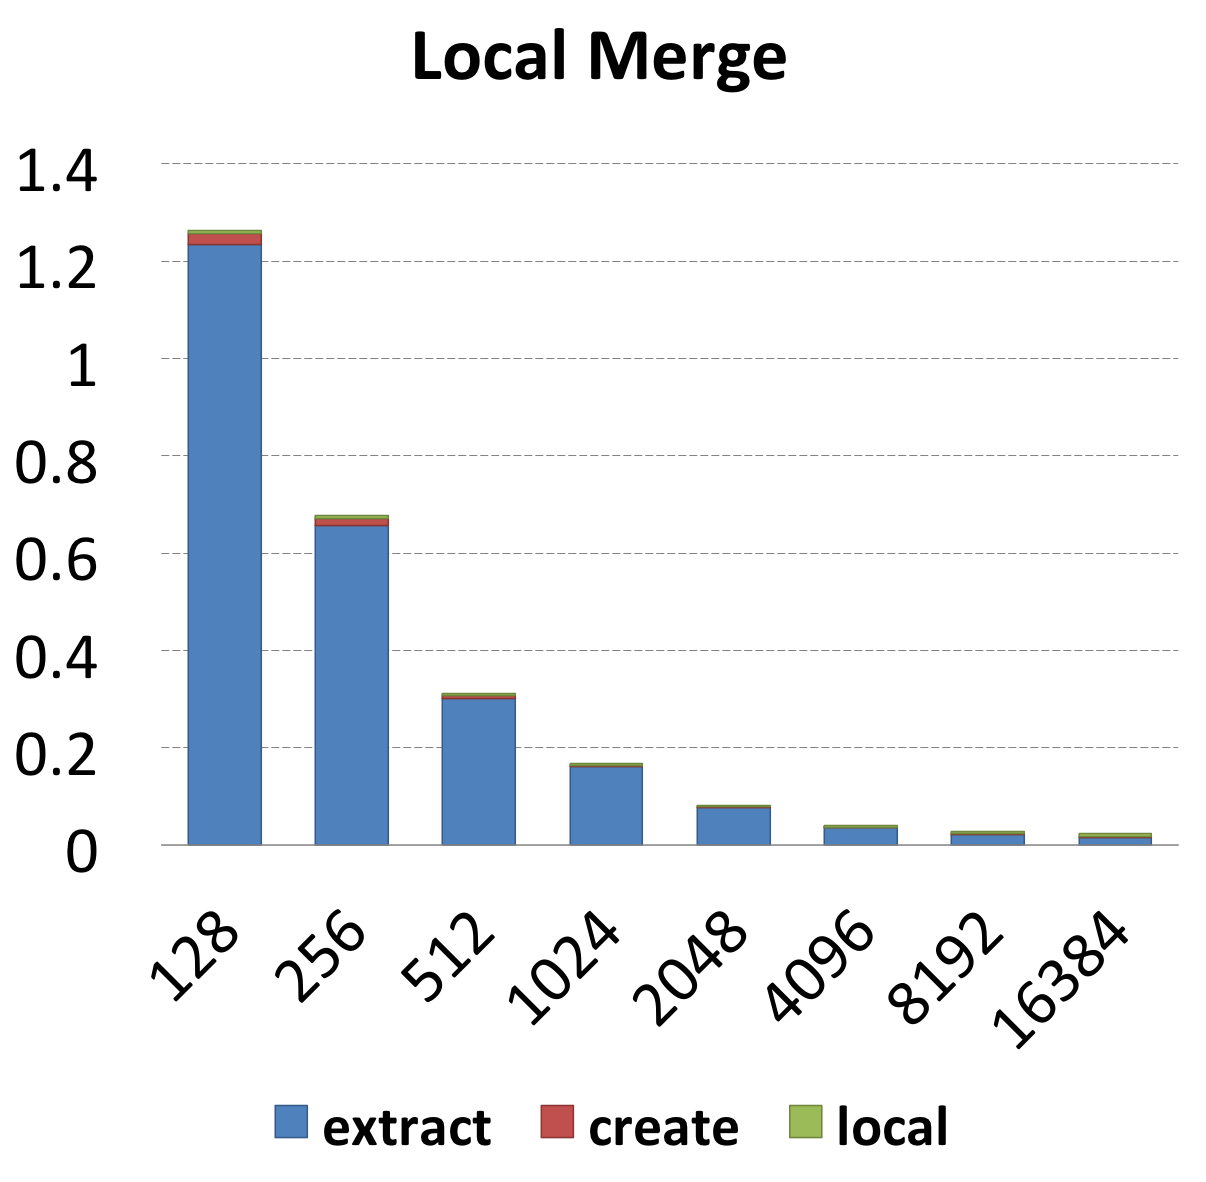
\includegraphics[width=1.0\linewidth]{local_merge.png}
\caption{Total computation time comparison for different approaches to global connectivity information generation. The centralized approach scales up to 2048 processors but the merging time outweighs the extraction time when using more processors; The decentralized approach scales linearly up 16384 processors for the combustion data set.}
\label{fig:global-merge}
\end{figure}

\textbf{Create Global Connectivity Information ($T_{merge}$)}
%
We also test the centralized approach and the decentralized approach in creating global connectivity information that is the major factor related to the scalability of our algorithm. Though the number of features-on-boundary decreases as more processors involved, the communication time for the centralized approach increases as $N_p$ increases. According to the comparison depicted in Figure~\ref{fig:local-vs-global}, we can see that the centralized approach is suitable for the scenarios that we only need a small number of processors, and the decentralized approach for creating connectivity information using a relatively large amount of the processors.

As shown in Figure~\ref{fig:global-merge}, the total time $T_{merge}$ for the centralized approach exceeds $T_{extract}$ after certain amount of processors, 2048, for the combustion data set, which makes the overall execution time rebounds . On the other hand, the decentralized approach  scales well up to 16384 processors for the combustion data set, as the communication cost is as low as ${O(\sqrt[3]{N_p})}$.
%------------------------------------------------------------------------------

%------------------------------------------------------------------------------
\section{Conclusion}

We present a scalable approach to extracting and tracking features for large time-varying 3D volume data using parallel machines. We carefully design the communication scheme such that only minimal amount data need to be exchanged among processors through local communication. The features are tracked in parallel by incrementally updating the connectivity information over time. Compared to the exiting solutions, our approach can significantly reduce  communication cost and ensure the scalability with up to 16384 processors. To the best of our knowledge, no prior approaches can extract and track features at the scale in terms of the number of processors we have achieved. 

In the future, we plan to integrate our approach with large scientific simulations and conduct experimental studies on in situ feature extraction and tracking. %to extract and track features during the simulation time. 
The study can possibly enable scientists to capture highly intermittent transient phenomena which could be missed in post-processing. In addition, we would like to investigate the feature-base data reduction and compression techniques to significantly reduce simulation data but retain the essential features for scientific discovery. Our parallel feature extraction and tracking approach builds a solid foundation for these future studies.   

% In this paper, we presented a decentralized approach that all feature connectivity information are created and preserved among distributed processors. Traditional approaches perform connectivity test on each processor and subsequently correspond them in a host processor after gathering all or partially merged connectivity information. Our approach does not follow this paradigm. Rather, instead being sent back to the host, the local connectivity information are computed and preserved only in the local processor.
% There is no copy of the global feature information preserved in the host, and the host only acts as the interface from where the criterion of feature of interest is broadcast. In this way, the computation of merging local connectivity information is distributed to the slaves, which can effectively remove the potential communication bottleneck on the host processor.
% Moreover, there's no need to set a barrier and wait for all connectivity information being sent back to the host, thus if one of the features spans over a large number of processors but was not selected by the user, the potentially long computation time for this feature will not be considered. This makes it ideal for an interactive system, where users can select the feature of interest and instantly receive the visual feedback as the feature evolves.
%------------------------------------------------------------------------------

%------------------------------------------------------------------------------
\bibliographystyle{eg-alpha-doi}
\bibliography{ptrack}

\end{document}
